\subsection{Behaviour of Model under Parameter Changes}
\label{sec:og.param.effects}

In this section, we examine the effects of the parameters on the function of the original model.
Starting with the combined effects of the parameters along areas of the same period.
And then also the individual effects of either parameter.

\subsubsection{Combined Effects of Parameters}

To replicate the dynamics seen in the model, it is helpful to know, how the model changes along the areas of the same period.
\Cref{fig:yunus.function.evolution.12} shows, how the model function changes along the area of period 12.
In the figure, there are three functions in three different colors.
The first function is blue and it is the model with parameters $E_0 = 15.9, \chi_0 = 0.11$, it is marked as point $A_12$ in \Cref{fig:yunus.function.evolution.map}.
The second function is purple and it is the model at the point $E_0 = 17.07, \chi_0 = 0.182$, marked as point $B_{12}$.
The last function is red and it is the model with parameters $E_0 = 18.5, \chi_0 = 0.27$, marked as point $C_{12}$.

\begin{figure}
    \centering
    \begin{subfigure}{0.4\textwidth}
        \includegraphics[width=\textwidth]{99_Yunus/2D_Period_Zoomed_Effects/result.png}
        \caption{Measured Points}
        \label{fig:yunus.function.evolution.map}
    \end{subfigure}
    \begin{subfigure}{0.4\textwidth}
        \includegraphics[width=\textwidth]{99_Yunus/ParameterEffects/E0_hi_P12/illustration.png}
        \caption{Evolution for Period 12}
        \label{fig:yunus.function.evolution.12}
    \end{subfigure}
    \begin{subfigure}{0.4\textwidth}
        \includegraphics[width=\textwidth]{99_Yunus/ParameterEffects/E0_hi_P10/illustration.png}
        \caption{Evolution for Period 10}
        \label{fig:yunus.function.evolution.10}
    \end{subfigure}
    \begin{subfigure}{0.4\textwidth}
        \includegraphics[width=\textwidth]{99_Yunus/ParameterEffects/E0_hi_P08/illustration.png}
        \caption{Evolution for Period 8}
        \label{fig:yunus.function.evolution.08}
    \end{subfigure}
    \caption{Effects of the Parameters on the Original Funtion}
\end{figure}

The most notable changes are
\begin{enumerate*}
    \item Branches $\A$ and $\C$ move upwards while the left part moves upwards more
    \item The left part of branches $\B$ and $\D$ move downwards 
    \item The local minima of these branches move to the left and downwards.
\end{enumerate*}
Smaller changes include
\begin{enumerate*}
    \item The border between branches $\B$ and $\C$ moves left
    \item The border between branches $\A$ and $\B$ moves right.
\end{enumerate*}
Note that regarding the borders, what happens to the border from $\B$ to $\C$, also applies to the border from $\D$ to $\A$.
Analogous for the borders from $\A$ to $\B$ and from $\C$ to $\D$ respectively.

The same effects can be observed for the areas of period 8 and 10.
The effects are visualized in \Cref{fig:yunus.function.evolution.10,fig:yunus.function.evolution.08}.
The points used for measurement are visualized in \Cref{fig:yunus.function.evolution.map}.
For the period 10, points $A_{10}, B_{10},$ and $C_{10}$ are used and for period 8, points $B_8$ and $C_8$.

\subsubsection{Individual Effects of Parameters}

The effects of the parameters described above, always include a change in both parameters $E_0$ and $\chi_0$.
To reproduce the bifurcation structures, it is important to know which effects on the function each parameter has individually.

For the parameter $E_0$, we fixed $\chi_0 = 0.2$ and varied $E_0$ in the parameter range $[15, 19]$, it is marked as the green arrow in \Cref{fig:yunus.function.evolution.single.map}.
Like before, we took the function at three points and put them in one figure with color codes.
\Cref{fig:yunus.function.evolution.e0} shows this.
The blue function is the function of the original model at the start of the parameter range, $E_0 = 15$ and $\chi_0 = 0.2$.
The purple function is in the middle at $E_0 = 17$, $\chi_0$ stays the same.
And the red function is at the end at $E_0 = 19$.
From the figure we can see three effects, the parameter has on the function of the original model in this parameter area.
The observed changes are
\begin{enumerate*}
    \item The left part of branches $\B$ and $\D$ move downwards
    \item The local minima of these branches move to the left and downwards
    \item The border between branches $\A$ and $\B$ moves right (also border between branches $\C$ and $\D$)
    \item The Right side of branches $\A$ and $C$ move up \todo{more precise since moves down for previous border location etc.}
\end{enumerate*}

\begin{figure}
    \centering
    \includegraphics[width=0.4\textwidth]{99_Yunus/2D_Period_Zoomed_EffectsSingle/result.png}
    \label{fig:yunus.function.evolution.single.map}
    \caption{Parameter Ranges Scanned for Individual Effects of Parameters}
\end{figure}

\begin{figure}
    \centering
    \begin{subfigure}{0.4\textwidth}
        \includegraphics[width=\textwidth]{99_Yunus/ParameterEffects/E0/illustration.png}
        \caption{Evolution for Parameter $E_0$}
        \label{fig:yunus.function.evolution.e0}
    \end{subfigure}
    \begin{subfigure}{0.4\textwidth}
        \includegraphics[width=\textwidth]{99_Yunus/ParameterEffects/hi/illustration.png}
        \caption{Evolution for Parameter $\chi_0$}
        \label{fig:yunus.function.evolution.hi}
    \end{subfigure}
    \caption{Effects of the Individual Parameters on the Original Funtion}
\end{figure}
